\documentclass[12pt]{article}

%useful packages
\usepackage{color,soul}
\usepackage[usenames,dvipsnames,svgnames,table]{xcolor}
\usepackage{amsmath,amsthm,amscd,amssymb,bm}
\usepackage{hyperref}
\hypersetup{
    colorlinks=true,
    linkcolor=JungleGreen
}
\usepackage[utf8]{inputenc}
\usepackage[top=2cm, bottom=3cm, left=2cm, right=2cm]{geometry}
\usepackage{pgfplots}
\usepackage{enumitem}
\usepgfplotslibrary{fillbetween}
\usetikzlibrary{patterns}
\usepackage{tcolorbox}
\usepackage{centernot}
\usepackage{mathtools}
\usepackage{xcolor}

%personal definitions and commands
\newcommand{\R}{\mathbb{R}} 
\newcommand{\E}{\mathbb{E}}
\newcommand{\V}{\mathbb{V}}
\newcommand{\C}{\mathbb{C}}
\newcommand{\Prob}{\mathbb{P}}
\newcommand{\e}{\epsilon}
\newcommand\numberthis{\addtocounter{equation}{1}\tag{\theequation}} %allows numbering of single equations in align* environment
\newcommand{\mtx}[1]{\ensuremath{\bm{\mathit{#1}}}}
\newcommand{\B}{\hat{\boldsymbol{\beta}}}
\newcommand{\Cov}{\mathbb{C}\text{ov}}
\newcommand{\N}{\mathcal{N}}



\title{ECON641 -- Problem Set 1}
\author{Anirudh Yadav}
\setlength\parindent{0pt}
\begin{document}

\maketitle

\setcounter{tocdepth}{1}
\tableofcontents

\newpage

\section{Warmup: factor intensity reversals}
First, I outline the small open economy environment of the $2\times 2$ HO model (for my own purposes). 
\begin{itemize}
\item Two goods, 1 and 2.
\item Two factors, $L$ and $K$; with endogenous factor prices $w$ and $r$, respectively.
\item Production technology is the same in both industries, but they may differ in their relative factor intensities.
\item Exogenously given goods prices, $p_1$ and $p_2$ (i.e. the demand side of the economy is pinned down).
\end{itemize}
Roughly speaking, `no factor intensity reversals' (NFIR) means the following: for any vector of factor prices $(w,r)$, the ordering of relative factor intensities in both industries is always the same. For example, in equilibrium the production of good 1 may be more capital intensive than production of good 2; NFIR implies that at any other vector of factor prices, the production of good 1 must always be more capital intensive compared to good 2. We can show that production technology exhibits NFIR if, given $p_1$ and $p_2$, equilibrium factor prices are uniquely pinned down.\\

\subsection{Cobb Douglas}

Cobb Douglas production clearly satisfies NFIR. To see this, suppose that $F_1(K_1,L_1) = AK_1^\alpha L_1^{1-\alpha}$ and $F_2(K_2,L_2) = AK_2^\beta L_2^{1-\beta}$. The first order conditions for the profit maximization problem for industry 1 are standard:
\begin{align}
p_1\alpha AK_1^{\alpha-1}L_1^{1-\alpha} &= r,\\
p_1(1-\alpha) AK_1^{\alpha}L_1^{-\alpha} &= w.
\end{align}
Dividing (2) by (1) gives
\begin{align}
\frac{1-\alpha}{\alpha} k_1 = \frac{w}{r} \implies k_1 = \frac{\alpha}{1-\alpha}\frac{w}{r}, \text{ where } k_1 = K_1/L_1 \label{eq:cd1}
\end{align}
Now, the zero profit condition in industry 1 is
\begin{align}
rK_1 + w L_1 &= p_1  AK_1^\alpha L_1^{1-\alpha} \nonumber\\
\implies r k_1 + w &= p_1 A k_1^\alpha
\end{align}
Plugging (3) into (4) and rearranging gives
\begin{align}
p_1 = C_\alpha r^\alpha w^{1-\alpha}
\end{align}
where $C_\alpha = \frac{1}{A(1-\alpha)}\left(\frac{1-\alpha}{\alpha}\right)^\alpha$. An analogous derivation for industry 2 gives
\begin{align}
p_2 = C_\beta r^\beta w^{1-\beta}
\end{align}
where $C_\beta = \frac{1}{A(1-\beta)}\left(\frac{1-\beta}{\beta}\right)^\beta$.
Clearly, given $p_1$ and $p_2$, there is a unique solution to (5) and (6), $(w^*,r^*)$, (unless $\alpha = \beta$).\\

Another (perhaps more intuitive) way to establish NFIR would be to use equation (3) and the equivalent expression for industry 2. These expressions imply that in equilibrium:
\begin{align*}
\frac{k_1}{k_2} = \frac{\alpha (1-\beta)}{\beta(1-\alpha)}.
\end{align*}
That is, the relative factor intensities between the two industries is independent of factor prices.\\


\subsection{CES}

CES production \textit{does not} exhibit NFIR. To see this, suppose $F_i(K_i,L_i) = \left[K_i^{\frac{\sigma_i - 1}{\sigma_i}} + L_i^{\frac{\sigma_i - 1}{\sigma_i}}\right]^{\frac{\sigma_i}{\sigma_i - 1}}$ for $i = 1,2$. The FOCs for industry $i$ are
\begin{align}
p_i\left[K_i^{\frac{\sigma_i - 1}{\sigma_i}} + L_i^{\frac{\sigma_i - 1}{\sigma_i}}\right]^{\frac{1}{\sigma_i - 1}}K_i^{-1/\sigma_i} &= r \label{eq:ces1}\\
p_i\left[K_i^{\frac{\sigma_i - 1}{\sigma_i}} + L_i^{\frac{\sigma_i - 1}{\sigma_i}}\right]^{\frac{1}{\sigma_i - 1}}L_i^{-1/\sigma_i} &= w \label{eq:ces1}
\end{align}
Combining these expressions gives
\begin{align*}
k_i^{-1/\sigma_i} &= \frac{r}{w}\\
\implies k_i &= \left(\frac{r}{w}\right)^{-\sigma_i}.
\end{align*}
Thus, in equilibrium, the relative factor intensities between the two industries is
\begin{align*}
\frac{k_1}{k_2} = \left(\frac{r}{w}\right)^{\sigma_2-\sigma_1},
\end{align*}
which clearly depends on factor prices (unless $\sigma_1 = \sigma_2$).\\

\subsection{Leontief}

Clearly the Leontief production function exhibits NFIR. Suppose both industries have the same production function $F(K,L) = \min\{K,L\}$. Then in equilibrium, both industries must have $k_i = 1$. Then, relative factor intensities do not depend on factor prices. More generally, suppose $F_i(K_i,L_i) = \min\{\alpha_iK,\beta_iL\}$. Then in equilibrium, each industry's capital-labor ratio will be $k_i = \beta_i/\alpha_i$. Again, relative factor intensities are independent of factor prices.

\newpage

\section{$2 \times 2 \times 2$ HO Model}

\subsection{Integrated equilibrium}
Integrated equilibrium is the competitive equilibrium that would prevail if both factors and goods were freely traded across countries. Thus, to solve for integrated equilibrium quantities and prices I simply assume that there is a representative consumer that maximizes utility subject to their (world) income, both firms maximize profits, and markets clear. I want to get expressions for equilibrium quantities $\{C_A,C_B,X_A,X_B,K_A,K_B,L_A,L_B\}$ and prices $\{p_A,p_B,w,r\}$, so I need to derive 12 equations that represent the equilibrium, make a suitable normalization and then do a lot of algebra. \\

Denote world endowments of labor and capital as $\bar L$ and $\bar K$, respectively. Start with the consumer's problem because it is easy. The consumer solves
\begin{align*}
\max_{C_A,C_B} U(C_A, C_B) \text{ s.t. } p_AC_A + p_BC_B = w\bar L + r\bar K.
\end{align*}
Given Cobb-Douglas preferences, it is easy to arrive at the demand functions:
\begin{align}
C_A &= \frac{1}{p_A} \alpha (w\bar L + r\bar K) \label{eq:HO1}\\
C_B &= \frac{1}{p_B} (1-\alpha) (w\bar L + r\bar K). \label{eq:HO2}
\end{align}
Next, consider the firms' profit maximization problems. I can skip a few steps here by using the results form Question 1 [1]. Combining the FOCs from the firms' maximization problems with the zero profit conditions gives expressions for goods prices in terms of factor prices:
\begin{align}
p_A &= \lambda_A r^{\beta_A}w^{1-\beta_A} \label{eq:HO3}\\
p_B &= \lambda_B r^{\beta_B}w^{1-\beta_B} \label{eq:HO4}
\end{align}
where $\lambda_i =  \frac{1}{(1-\beta_i)}\left(\frac{1-\beta_i}{\beta_i}\right)^{\beta_i}$ for $i = A,B$.\\

Next, I derive the unit factor requirements for both goods, which I'll use later in the market clearing conditions. To do so, I solve the firms' cost minimization problems. Firm $i$ solves
\begin{align*}
\min_{K_i,L_i} rK_i + wL_i \text{ s.t } K_i^{\beta_i}L_i^{1-\beta_i} \geq 1
\end{align*}
Again, I can skip a lot of the math because it is almost identical to that in Question 1 [1]. Each firm chooses its capital/labor ratio such that
\begin{align*}
\frac{K_i}{L_i} = \frac{\beta_i}{1-\beta_i}\left(\frac{w}{r}\right).
\end{align*}
Plugging this expression into the production function gives unit factor requirements for each sector. For labor:
\begin{align}
\left[ \frac{\beta_i}{1-\beta_i}\left(\frac{w}{r}\right)\right]^{\beta_i} L_i &= 1 \nonumber \\
\implies L_i \equiv a_{L,i}(w,r) =  \left[ \frac{\beta_i}{1-\beta_i}\left(\frac{w}{r}\right)\right]^{-\beta_i} \label{eq:HO5}
\end{align}
Similarly, the unit capital requirement for sector $i$ is
\begin{align}
a_{K,i} =  \left[ \frac{\beta_i}{1-\beta_i}\left(\frac{w}{r}\right)\right]^{1-\beta_i} \label{eq:HO6}
\end{align}
Then, factor demands are given by
\begin{align}
L_i &= a_{L,i}(w,r) X_i \label{eq:HO7}\\
K_i &= a_{K,i}(w,r) X_i \label{eq:HO8}
\end{align}
for $i = A,B$. Finally the market clearing conditions are:
\begin{align}
X_i &= C_i, \text{ for } i = A,B  \label{eq:HO9}\\
L_A + L_B &= \bar L \label{eq:HO10}\\
K_A + K_B &= \bar K. \label{eq:HO11}
\end{align}
Equations (\ref{eq:HO1})--(\ref{eq:HO11}) fully characterize the integrated equilibrium. Next, I need to do a lot of algebra to get expressions for equilibrium quantities and prices. Start with the labor market clearing condition
\begin{align*}
a_{L,A}(w,r) X_A+ a_{L,B}(w,r) X_B =\bar L
\end{align*}
Then, use the goods market clearing conditions, and plug in the demand functions (\ref{eq:HO1}) and (\ref{eq:HO2}) to get
\begin{align*}
 \bar L&=a_{L,A}(w,r) \frac{\alpha}{p_A}(w\bar L + r\bar K) + a_{L,B}(w,r)\frac{1-\alpha}{p_B}(w\bar L + r\bar K) \\
 &=(w\bar L + r\bar K)\left[a_{L,A}(w,r) \frac{\alpha}{p_A} + a_{L,B}(w,r)\frac{1-\alpha}{p_B}\right].
\end{align*}
Next, plug in the unit labor requirements (\ref{eq:HO5}) and goods prices (\ref{eq:HO3}) and (\ref{eq:HO4}):
\begin{align*}
 \bar L&= (w\bar L + r\bar K)\left[\left[ \frac{\beta_A}{1-\beta_A}\left(\frac{w}{r}\right)\right]^{-\beta_A} \frac{\alpha}{\lambda_A r^{\beta_A}w^{1-\beta_A} } + \left[ \frac{\beta_B}{1-\beta_B}\left(\frac{w}{r}\right)\right]^{-\beta_B}  \frac{1-\alpha}{\lambda_B r^{\beta_B}w^{1-\beta_B} }\right].
\end{align*}
This is an ugly expression, so it seems like the appropriate time to make the normalization $w = 1$. Plugging in the constants, $\lambda_A$ and $\lambda_B$ also helps to simplify the above expression; I get:
\begin{align*}
 \bar L&= (\bar L + r\bar K)\left[\alpha(1-\beta_A) + (1-\alpha)(1-\beta_B)\right],
\end{align*}
which looks much better (phew!). Now, solving for $r$ gives
\begin{align}
r^* = \left[\frac{\alpha\beta_A + (1-\alpha)\beta_B}{\alpha(1-\beta_A) + (1-\alpha)(1-\beta_B)}\right] \frac{\bar L}{\bar K} \label{eq:12}
\end{align}
and I'm essentially done. By Walras' law the capital market also clears. To get equilibrium goods prices, $p^*_A$ and $p^*_B$, plug $r^*$ into (\ref{eq:HO3}) and (\ref{eq:HO4}). Then plug these equilibrium prices into (\ref{eq:HO1}) and (\ref{eq:HO2}) to get equilibrium consumption $C_A^*$ and $C_B^*$, which in turn give $X_A^*$ and $X_B^*$ via goods market clearing. Finally, plug in $r^*$ and $X_i^*$ into (\ref{eq:HO7}) and (\ref{eq:HO8}) to get the equilibrium quantities of labor and capital used in each sector.

\subsection{FPE set}
The FPE set is the set of country factor endowment pairs $((L_H,K_H),(L_F,K_F))$ such that every country can fully employ its factors and $w_H=w_F, r_H=r_F$. The idea is that factor prices will be equalized under free trade of goods (not factors) if the countries' endowments are not too dissimilar.\\

The integrated equilibrium factor demands for each sector are
\begin{align*}
L^*_A &= \left[\frac{\alpha(1-\beta_A) }{\alpha(1-\beta_A) + (1-\alpha)(1-\beta_B)}\right] \bar L\\
L^*_B &= \bar L - L^*_A\\
K^*_A &=  \left[\frac{\alpha\beta_A}{\alpha\beta_A + (1-\alpha)\beta_B}\right] \bar K\\
K^*_B &= \bar K - K^*_A
\end{align*}

I plot the FPE set for the given parameters below; Home's `origin' is at the lower left corner. The endowment vector is represented by the red dot; clearly, it is not in the FPE set.

\begin{figure}[!htpb]
    \centering
    
        %\centering
        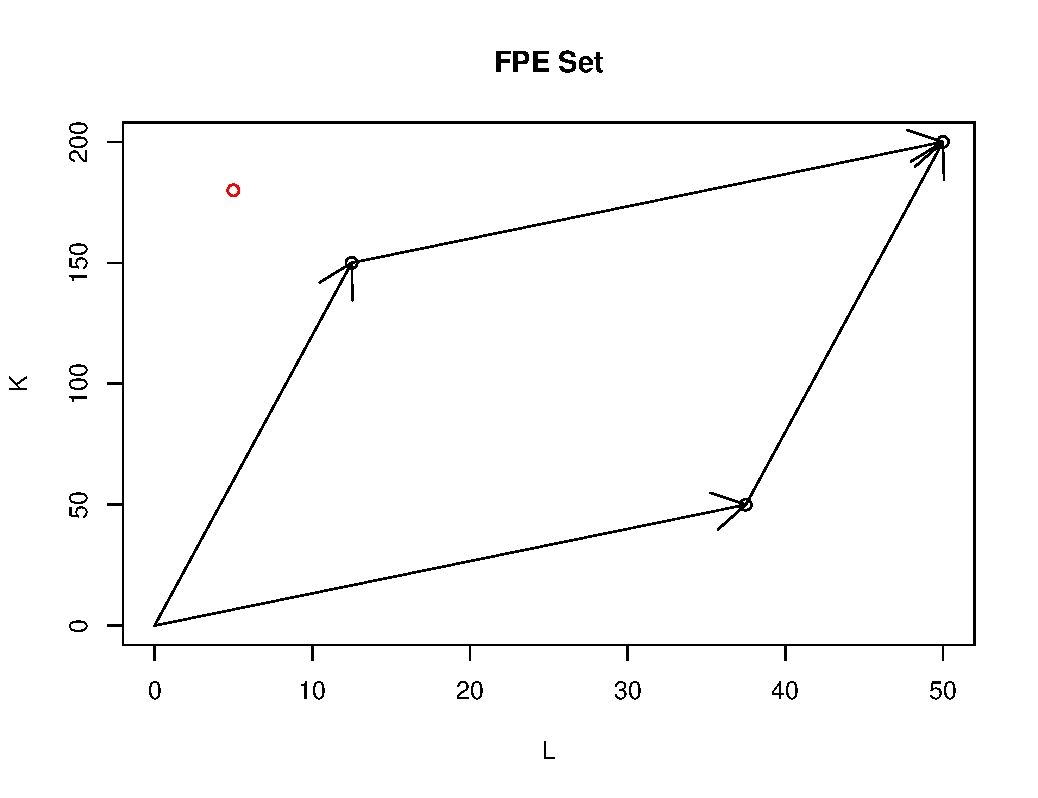
\includegraphics[width=0.7\textwidth]{fpeset.pdf}

\end{figure}

\subsection{Autarky}
Autarkic equilibrium prices and quanties in both countries look very similar to their integrated equilibrium counterparts, except with different factor endowments. With the normalization $w^j = 1$ for $j = H,F$, the same algebra as in the integrated equilibrium case gives the autarkic rental rates:
\begin{align*}
r^j = \left[\frac{\alpha\beta_A + (1-\alpha)\beta_B}{\alpha(1-\beta_A) + (1-\alpha)(1-\beta_B)}\right] \frac{L^j}{K^j}.
\end{align*}
Again, for brevity, I won't derive expressions for autarkic goods prices and quantities; but to do so, I would simply use the same procedure as noted in integrated equilibrium case.  \\

Now, consider the case where trade in goods is not allowed but labor is fully mobile across countries (i.e. free immigration). In this case, there is a single `world' labor market clearing condition:
\begin{align}
a_{L,A}(w^H,r^H) X^H_A+ a_{L,B}(w^H,r^H) X^H_B + a_{L,A}(w^F,r^F) X^F_A+ a_{L,B}(w^F,r^F) X^F_B=\bar L \label{eq:aut1}
\end{align}
Now, autarky equilibrium is a set of quantities $\{C^j_A,C^j_B,X^j_A,X^j_B,K^j_A,K^j_B,L^j_A,L^j_B\}_j$ and prices $\{p^j_A,p^j_B,w^j,r^j\}_j$ that solve the following system of equations along with the labor market clearing condition (\ref{eq:aut1})
\begin{align*}
\alpha  &= {\frac{p_A^jX_A^j}{p^j_AX_A^j + p_B^jX_B^j}}\\
p^j_A &= \lambda_A r_j^{\beta_A}w_j^{1-\beta_A} \\
p^j_B &= \lambda_B r_j^{\beta_B}w_j^{1-\beta_B} \\
K^j_i &= a_{K,i}(w^j,r^j) X^j_i  \text{ for } i = A,B \\
X^j_i &= C^j_i, \text{ for } i = A,B \\
K^j_A + K^j_B &= K^j\\
L_i^j &= a_{L,i}(w^j,r^j) X^j_i+ a_{L,i}(w^j,r^j) X^j_i \text{ for } i = A,B
\end{align*}
for $j = H,F$ (note that this is a system of 21 equations in 21 endogenous variables). This looks like a tough problem to solve, but note that with free immigration, in equilibrium the real wage will be equalized across both countries; that is
\begin{align}
\frac{w^H}{P^H} = \frac{w^F}{P^F} \label{eq:aut2}
\end{align}
where $P^j$ is the ideal aggregate price index
\begin{align*}
P^j = \frac{(p_A^j)^\alpha(p_B^j)^{1-\alpha}}{\alpha (1-\alpha)} \text{ for } j = H,F.
\end{align*}
Next, I use the fact that in equilibrium, goods prices equal the unit cost of production. Plugging these expressions for goods prices into (\ref{eq:aut2}) with the given parameters gives
\begin{align*}
\left(\frac{w^H}{r^H}\right)^{1/2} = \left(\frac{w^F}{r^F}\right)^{1/2},
\end{align*}
which says that factor prices are equalized with free immigration. Then, using equation (\ref{eq:cd1}) from Question 1, I know that factor intensities for each industry are also equalized across countries in equilibrium. Now, I'm done. Since factor intensities are equalized in equilibrium, I can easily back out the required level of immigration from Foreign to Home:
\begin{align*}
\frac{K^H}{L^H + L^{\texttt{migrate}}} = \frac{K^F}{L^F - L^{\texttt{migrate}}} \implies L^{\texttt{migrate}}=40.
\end{align*}

\subsection{Free trade}


\newpage

\section{Monopolistic competition with variable markups}

\subsection{Consumer's problem}
The consumer's problem is 
\begin{align*}
&\max_{q_i} \int_0^N (1-\exp(-\alpha q_i) )di\\
&\text{s.t.} \int_0^N p_i q_i di = E.
\end{align*}
The Lagrangian is
\begin{align*}
\mathcal{L} &=  \int_0^N (1-\exp(-\alpha q_i)) di + \lambda \left[ E -\int_0^N p_i q_i di \right].
\end{align*}
The FOC wrt variety $i$ is
\begin{align*}
\alpha \exp(-\alpha q_i) = \lambda p_i
\end{align*}
Since this FOC holds for all varieties, for any pair of varieties $i, j$ I can take the ratio
\begin{align*}
\frac{\alpha \exp(-\alpha q_i)}{\alpha \exp(-\alpha q_j)} & = \frac{\lambda p_i}{\lambda p_j}
\end{align*}
Rearranging this expression gives demand for good $i$ as a function of demand for good $j$ and their respective prices:
\begin{align}
q_i = q_j - \frac{1}{\alpha} \log\left(\frac{p_i}{p_j}\right). \label{eq:mpc1}
\end{align}
To derive the demand for good $i$ as a function of $E$ and goods prices only, multiply both sides of the above expression by $p_j$ and then integrate over $j$:
\begin{align}
\int_0^N q_i p_j dj &= E - \frac{1}{\alpha}\int_0^N \log\left(\frac{p_i}{p_j}\right)p_j dj \nonumber\\
\therefore q_i &=  \frac{E - \frac{1}{\alpha}\int_0^N \log\left(\frac{p_i}{p_j}\right)p_j dj}{\int_0^Np_j dj} \label{eq:mpc2a}
\end{align}


\subsection{Firm's problem}
\textbf{[1] }Firm $i$'s profit maximization problem is
\begin{align*}
&\max_{p_i,q_i} Lq_i(p_i - mw)\\
& \text{s.t. (\ref{eq:mpc2a})}
\end{align*}
Plugging the firm's demand constraint into it's profit function allows me to rewrite the objective as
\begin{align*}
\max_{p_i} L \left[ \frac{E - \frac{1}{\alpha}\int_0^N \log\left(\frac{p_i}{p_j}\right)p_j dj}{\int_0^Np_j dj}\right](p_i - mw).
\end{align*}
The FOC is
\begin{align*}
\frac{E}{\int_0^Np_j dj} - \frac{1}{\alpha \int_0^Np_j dj} \frac{\partial}{\partial p_i}\left\{(p_i - mw)\int_0^N \log\left(\frac{p_i}{p_j}\right)p_j dj \right\} &=0\\
\implies \frac{\partial}{\partial p_i}\left\{(p_i - mw)\int_0^N \log\left(\frac{p_i}{p_j}\right)p_j dj \right\} &=\alpha E
\end{align*}
Now,
\begin{align*}
\frac{\partial}{\partial p_i}\left\{(p_i - mw)\int_0^N \log\left(\frac{p_i}{p_j}\right)p_j dj \right\} &=\frac{\partial}{\partial p_i}\left\{(p_i - mw)\int_0^N \log(p_i) p_j -\log (p_j)p_j dj \right\}\\
&= 1\cdot \log(p_i) \int_0^N  p_j dj + \frac{p_i - mw}{p_i}\int_0^N  p_j dj -\int_0^N \log (p_j)p_j dj\\
&=\int_0^N \log\left(\frac{p_i}{p_j}\right)p_j dj + \frac{p_i - mw}{p_i}\int_0^N  p_j dj
\end{align*}
Thus, the FOC for the firm's problem is
\begin{align}
\int_0^N \log\left(\frac{p_i}{p_j}\right)p_j dj + \frac{p_i - mw}{p_i}\int_0^N  p_j dj = \alpha E \label{eq:mpc3}
\end{align}

\textbf{[2]} Now, under symmetric equilibrium, $p_i = p_j \equiv p$ for all $i,j$. Thus, the FOC (\ref{eq:mpc3}) simplifies to
\begin{align}
\int_0^N \log\left(\frac{p}{p}\right)p dj + \frac{p - mw}{p}\int_0^N  p dj &= \alpha E \nonumber\\
\implies \frac{p - mw}{p} Np &= \alpha E\nonumber\\
\therefore p = mw + \frac{\alpha E}{N} \label{eq:mpc4}.
\end{align}
Thus, the optimal price features a markup over the marginal cost, which is decreasing in the number of firms. This result differs from the CES case, in which the optimal price features a constant markup over marginal costs (and does not depend on the number of firms).\\

\textbf{[3]} To get the equilibrium quantity of each good sold, plug the optimal price (\ref{eq:mpc4}) into the consumer's demand function (\ref{eq:mpc2a}):
\begin{align*}
q = \frac{E}{Np} &= \frac{E}{N}\left[  mw + \frac{\alpha E}{N}\right]^{-1}\\
&=\frac{E}{N} \frac{N}{mwN + \alpha E}\\
&= \frac{E}{mwN + \alpha E}
\end{align*}
And then, each firm's variable profit is
\begin{align}
\Pi_v &= Lq(p-mw) \nonumber\\
&= L\frac{E}{mwN + \alpha E}  \frac{\alpha E}{N} \nonumber\\
&=\frac{L}{N} \frac{\alpha E^2}{ mwN + \alpha E} \label{eq:mpc5}
\end{align}

\subsection{Equilibrium number of firms}
\textbf{[1]} The free entry condition implies
\begin{align*}
\Pi = \frac{L}{N} \frac{\alpha E^2}{ mwN + \alpha E}  - wF = 0
\end{align*}
Plugging in $E=w$ implies that in equilibrium 
\begin{align*}
w \left[ \frac{\alpha L}{N(mN+ \alpha)} - F\right] &= 0
\end{align*}
Solving for $N$ using the quadratic formula gives
\begin{align*}
N = \frac{-\alpha F + \sqrt{\alpha^2F^2 + 4(mF)(\alpha L)}}{2mF}.
\end{align*}

\textbf{[2]} Now, I can solve for welfare $w/p$ by using (\ref{eq:mpc4}) and plugging in $E=w$:
\begin{align*}
p &= mw + \frac{\alpha w}{N}\\
\implies \frac{w}{p} &=\frac{N}{\alpha + mN}
\end{align*}
Then
\begin{align*}
\frac{\partial}{\partial N} \frac{w}{p}  = \frac{\alpha}{(\alpha + mN)^2} >0 ,
\end{align*}
so welfare is increasing in the number of firms (for $\alpha > 0 $).

\newpage

\section{A simple model of institutional comparative advantage}

\newpage


\section{Technology growth in a parameterized version of DFS}

\subsection{}
I follow the derivation in EK (2005). We are given the distribution of efficiencies for producing goods $j$ at Home and Foreign:
\begin{align*}
F_i(z)=\Pr[Z_i(j) \leq z ] = \exp(-T_iz^{-\theta})
\end{align*}

\iffalse
Now, if we pick some random $j \in [0,1]$, the probability distribution of its efficiency, $Z_i(j)$, is obviously same as above. Accordingly, we can order goods such that
\begin{align*}
j &= \exp(-T_iz_i(j)^{-\theta})\\
\implies z_i(j) &= \left(-\frac{T_i}{\ln j}\right)^{-1/\theta}.
\end{align*}
(Essentially, think of the index $j$ as the vertical axis of the CDF above).\\
\fi


Now, we want to derive the DFS-type $A(j)$ curve, which is defined as the ratio of $H$'s efficiency of producing $j$ to $F$'s corresponding efficiency.\\

In the EK setup the efficiencies are realizations of a random variable. Accordingly, we think of $j$ as the \textit{probability} that the $H$'s relative efficiency of producing $j$ is less than some number:
\begin{align*}
j &= \Pr\left[\frac{Z}{Z^*} \leq A\right]\\
&=\Pr\left[Z \leq AZ^*\right]\\
&= \int_0^\infty \exp(-T(Az_*)^{-\theta}) f(z_*)dz_*.
\end{align*}
Now,
\begin{align*}
f(z_*) = \frac{d}{dz} \exp(-T^*z^{-\theta}) = \theta T^*z^{-\theta-1}\exp(-T^*z^{-\theta})
\end{align*}
Substituting into the above integral gives
\begin{align*}
j &= T^*\int_0^\infty \exp(-T(Az_*)^{-\theta}) \times \theta z_*^{-\theta-1}\exp(-T^*z_*^{-\theta})dz_*\\
&=T^*\int_0^\infty \exp(-(TA^{-\theta}+T^*)z_*^{-\theta}) \times\theta z_*^{-\theta-1}dz_*\\
&= \frac{T^*}{(TA^{-\theta}+T^*)} \int_0^\infty \exp(-(TA^{-\theta}+T^*)z_*^{-\theta}) \times -\theta z_*^{-\theta-1}(TA^{-\theta}+T^*)dz_*\\
&=\frac{T^*}{(TA^{-\theta}+T^*)} \int_0^\infty \exp(-(TA^{-\theta}+T^*)z_*^{-\theta}) \times \theta z_*^{-\theta-1}(TA^{-\theta}+T^*)dz_*\\
&=\frac{T^*}{(TA^{-\theta}+T^*)},
\end{align*}
since $ \int_0^\infty \exp(-(TA^{-\theta}+T^*)z_*^{-\theta}) \times \theta z_*^{-\theta-1}(TA^{-\theta}+T^*)dz_* = 1$ (because it is the integral of the Frechet pdf with scale $(T^*A^{-\theta}+T)$). Thus, rearranging to get an expression for $A(j)$ gives
\begin{align}
A(j) = \left[\left(\frac{1-j}{j}\right)\frac{T^*}{T}\right]^{-1/\theta}. \label{eq:EK0}
\end{align}

\newpage

\subsection{}
First note that there are no trade costs so that $d_{ni} = 1$ for all $n,i \in \{F,H\}$.\\

Now, we know that within a country, goods will be purchased from the lowest cost source. Since Home has a comparative advantage at lower values of $j$, we know that Home will produce the range of goods $[0,\bar j]$ where
\begin{align*}
\frac{w}{z(\bar j)} = \frac{w^*}{z^*(\bar j)}.
\end{align*}
The LHS of the above expression is the unit cost of producing $\bar j$ at home, and the RHS is the cost of buying the good from Foreign. Rearranging the above expression gives
\begin{align}
\frac{z(\bar j)}{z^*(\bar j)} &= \frac{w}{w^*} \nonumber\\
\implies A(\bar j) &= \omega, \label{eq:EK1}
\end{align}
where $\omega = w/w^*$. Similarly, Foreign will produce a range of goods $[\underline j, 1]$ domestically, such that
\begin{align}
\frac{w^*}{z^*(\underline j)} &= \frac{w}{z(\underline j)} \nonumber \\
\implies A(\underline j) = \omega. \label{eq:EK2}
\end{align}
Thus, there is a unique cuttoff good.\\

Next, we need to invoke market clearing. Here, we note that preferences are Cobb Douglas, with equal weights across each good. Thus, each country spends a constant share of its income on each good. We know that Home produces $[0,\bar j]$ goods domestically, and exports $[0, \underline j]$ goods to Foreign. Thus, market clearing at Home requires
\begin{align}
wL = \bar j wL + \underline j w^*L^* \label{eq:EK3}\\
\end{align}
Substituting (\ref{eq:EK1}) and (\ref{eq:EK2}) into (\ref{eq:EK3}) and rearranging gives
\begin{align*}
L &= L A^{-1}(\omega) + \frac{1}{\omega} L^* A^{-1}(\omega)\\
\implies \frac{1}{A^{-1}(\omega)} &= 1 + \frac{1}{\omega} \frac{L^*}{L} 
\end{align*}
And, from the above derivation we know: $A^{-1}(\omega) = \frac{T^*}{(T\omega^{-\theta}+T^*)}$. Substituting this into the above expression gives
\begin{align*}
\frac{T\omega^{-\theta}+T^*}{T^*} &= 1 +\frac{1}{\omega} \frac{L^*}{L}\\
\implies \frac{T}{T^*} \omega^{-\theta} &=\frac{1}{\omega} \frac{L^*}{L}\\
\implies \omega &= \left[\frac{T^*}{T}\frac{L^*}{L}\right]^{1/(1-\theta)}.
\end{align*}
And the equilibrium cutoff good is
\begin{align*}
\bar j &= A^{-1}(\omega)
\end{align*}

\subsection{}
With no trade costs goods prices are identical in $H$ and $F$. Thus, $\omega$ measures $H$'s welfare relative to $F$'s. From the above expression for equilibrium $\omega$, if $\theta > 1$, then an increase in $T^*$ reduces relative welfare in $H$. The comparative static is
\begin{align*}
\frac{d\omega}{dT^*} = \left[\frac{1}{T}\frac{L^*}{L}\right]^{1/(1-\theta)} \frac{1}{1-\theta} (T^*)^{\theta/(1-\theta)}.
\end{align*}
So, if $\theta > 1$, then the effect of an increase in $T^*$ is decreasing in $L^*/L$, which is observable in the data.

\newpage

\section{Key implications of EK's Ricardian model}

\subsection{}
The unit cost of sending good $j$ from $i$ to $n$ is given by
\begin{align}
C_{ni}(j) = \frac{c_i}{Z_i(j)}d_{ni} \label{eq:EK21}
\end{align}

\subsection{}
We want to compute the probability that $i$ will sell good $j$ to $n$. Since the derivation below is the same for all goods, I suppress the index $j$. \\

\textbf{(a)} From (\ref{eq:EK21}) note that 
\begin{align*}
Z_i = \frac{c_id_{ni}}{C_{ni}}
\end{align*}
Now,
\begin{align*}
\Pr[Z_i \leq p] &= \Pr[{c_id_{ni}}/{C_{ni}} \leq p]
\end{align*}
Thus,
\begin{align*}
\Pr[Z_i \leq {c_id_{ni}}/{p} ] &=  \Pr[{c_id_{ni}}/{C_{ni}} \leq {c_id_{ni}}/{p}]\\
&= \Pr[p \leq C_{ni}]\\
&= \Pr[C_{ni} \geq p]\\
&= 1- \Pr[C_{ni} \leq p]\\
\therefore \Pr[C_{ni} \leq p] &= 1-\Pr[Z_i \leq {c_id_{ni}}/{p} ]\\
&= 1- F_i(c_id_{ni}/{p})\\
&= 1- \exp(-T_i(c_id_{ni})^{-\theta}p^\theta),
\end{align*}
which is the probability distribution of $C_{ni}$. Denote this distribution as $G_{ni}$ so that
\begin{align}
G_{ni}(p) = 1- \exp(-T_i(c_id_{ni})^{-\theta}p^\theta) \label{eq:EK22}
\end{align}

\textbf{(b)} Next we want to compute the probability that $i$ is the cheapest supplier for $n$. Denote this probability as $\pi_{ni}$. We have
\begin{align}
\pi_{ni} \equiv \Pr[ C_{ni} &= \min\{C_{ns}; s\neq i\}] \nonumber \\
&= \Pr[C_{ns} \geq C_{ni} \text{ for all } s \neq i]\nonumber \\ 
&= \int_0^\infty \prod_{s\neq i}[1-G_{ns}(C_{ni})] dG_{ni}(C_{ni})\nonumber \\
&=  \int_0^\infty \prod_{s\neq i}[1-G_{ns}(p)] dG_{ni}(p), \label{eq:EK23}
\end{align}
where I just re-denote the integration dummy as $p$ to ease notation.\\

\textbf{(c)} Now,
\begin{align}
dG_{ni}(p) = \frac{d}{dp} G_{ni}(p) &= \exp(-T_i(c_id_{ni})^{-\theta}p^\theta) T_i(c_id_{ni})^{-\theta} \theta p^{\theta-1} \label{eq:EK24}
\end{align}
Substituting (\ref{eq:EK22}) and (\ref{eq:EK24}) into (\ref{eq:EK23}) gives
\begin{align*}
\pi_{ni} &= \int_0^\infty\left[ \prod_{s\neq i} \exp(-T_s(c_sd_{ns})^{-\theta}p^\theta) \right] \exp(-T_i(c_id_{ni})^{-\theta}p^\theta) T_i(c_id_{ni})^{-\theta} \theta p^{\theta-1}dp\\
&=  \int_0^\infty\exp(-\sum_{s \neq i} T_s(c_sd_{ns})^{-\theta}p^\theta)  \exp(-T_i(c_id_{ni})^{-\theta}p^\theta) T_i(c_id_{ni})^{-\theta} \theta p^{\theta-1}dp\\
&= \int_0^\infty\exp(-\sum_{i=1}^N T_i(c_{ni}d_{ni})^{-\theta}p^\theta)T_i(c_id_{ni})^{-\theta} \theta p^{\theta-1}dp\\
&=\int_0^\infty\exp(-\Phi_np^\theta) T_i(c_id_{ni}) \theta p^{\theta-1}dp\\
&=T_i(c_id_{ni})^{-\theta} \int_0^\infty\exp(-\Phi_np^\theta) \theta p^{\theta-1}dp\\
&= \frac{T_i(c_id_{ni})^{-\theta} }{\Phi_n} \int_0^\infty\exp(-\Phi_np^\theta) \Phi_n\theta p^{\theta-1}dp\\
&=\frac{T_i(c_id_{ni})^{-\theta} }{\Phi_n},
\end{align*}
since the integral in the second last line evaluates to 1, because it is a pdf of a probability distribution of the form (\ref{eq:EK22}).

\subsection{} Next we want to compute the probability distribution of goods prices actually bought in market $n$. Call this price $P_n$ and recall that $n$ buys the lowest cost good
\begin{align*}
P_n = \min_{i=1,..,N}\{C_{ni}\}
\end{align*}
Thus
\begin{align*}
\Pr[P_n \leq p ] &= \Pr[ \min_{i=1,..,N}\{C_{ni}\} \leq p]\\
&= 1-\Pr[C_{ni} > p \text{ for all } i]\\
&= 1- \prod_{i=1}^N[1-G_{ni}(p)]\\
&= 1-  \prod_{i=1}^N \exp(-T_i(c_id_{ni})^{-\theta}p^\theta) \text{ using (\ref{eq:EK22}),}\\
&= 1- \exp(-\Phi_n p^\theta).
\end{align*}
Denote this distribution as $G_n(p)$, so that 
\begin{align}
G_n(p) \equiv \Pr[P_n \leq p ] = 1- \exp(-\Phi_n p^\theta) \label{eq:EK25}
\end{align}

\subsection{} Next, we want to compute the probability distribution of goods prices that $n$ \textit{actually buys} from country $i$. That is, we want to compute the conditional probability distribution:
\begin{align*}
\Pr[P_n \leq p | P_n = C_{ni}]
\end{align*}
Now,
\begin{align*}
Pr[P_n \leq p | P_n = C_{ni}]&=\Pr[P_n \leq p |C_{ni} = \min\{C_{ns}; s\neq i\}]\\
&=\Pr[C_{ni}  \leq p |C_{ni} = \min\{C_{ns}; s\neq i\}]\\
&=\frac{1}{\pi_{ni}} \int_0^p \prod_{s \neq i}  [1-G_{ns}(q)] dG_{ni}(q)\\
&=\frac{1}{\pi_{ni}} \pi_{ni}\int_0^p \exp(-\Phi_nq^\theta) \Phi_n\theta q^{\theta-1}dq,
\end{align*}
using our previous derivations. Thus,
\begin{align*}
\Pr[P_n \leq p | P_n = C_{ni}]&= \int_0^p \exp(-\Phi_nq^\theta) \Phi_n\theta q^{\theta-1}dq \\
&= \int_0^p dG_n(q)\\
&= G_n(p).
\end{align*}
So, for goods that are purchased in $n$, conditioning on the source does not affect the distribution of the good's price. This result seems at odds with reality, as we discussed in class. One would think that German cars bought in the US would have a different price distribution compared to Japanese cars bought in the US.


\subsection{}
I'm not exactly sure how to do this problem, but here's my best shot.\\

\textbf{(a)} Given CES preferences over the unit mass of goods, $n$'s demand for good $j$ is given by
\begin{align*}
X_n(j) &= \left(\frac{P_n(j)}{P_n}\right)^{1-\sigma}X_n\\
&=  \left(\frac{\min_{i=1,..,N}\{C_{ni}(j)\}}{P_n}\right)^{1-\sigma}X_n
\end{align*}

\textbf{(b)} Then, $n$'s expected expenditure on good $j$, sourced from $i$ is
\begin{align*}
X_{ni}(j) &= \E[X_n(j)  | i*(j) = i] \Pr[i^*(j) = i]\\
&=\E \left[\left(\frac{\min_{i=1,..,N}\{C_{ni}(j)\}}{P_n}\right)^{1-\sigma}X_n|  i^*(j) = i\right] \pi_{ni}\\
&= \E \left[\left(\frac{C_{ni}(j)}{P_n}\right)^{1-\sigma}X_n|  i^*(j) = i\right] \pi_{ni}\\
&= \E \left[\left(\frac{P_n}{P_n}\right)^{1-\sigma}X_n|  i^*(j) = i\right] \pi_{ni}\\
&= \pi_{ni} X_n.
\end{align*}




\subsection{} We've shown that $\pi_{ni}$ is the probability that country $n$ purchases good any good $j$ from $i$. Since there is a unit measure of goods, it follows that $\pi_{ni}$ is the total fraction of the $j \in [0,1]$ goods that are sourced from from $i$ in country $n$. Then, we can split the the total unit measure $j\in [0,1]$ of goods purchased in $n$ into the share supplied by each source country. Recall that conditioning on the source of a good does not affect the distribution of the good's price in $n$. Accordingly, the fraction of $n$'s total expenditure that goes to country $i$ is the same as the fraction of goods that $n$ purchases from country $i$; namely, $\pi_{ni}$.


\section{Quantitative analysis in the EK model}

\subsection{A peek at the data}
See attached \verb|R| code for the aggregation of the WIO data.\\

Table 1 (overleaf) shows the ratio of imports of intermediate goods to total imports for each country in the WIOD. For each country in the sample, imports of intermediate goods accounts for more than half of total imports; the mean intermediate import share is 0.64. These results imply that it is extremely important to incorporate and intermediate goods sector when modelling aggregate trade flows.\\

Table 2 presents the ratio of each country's trade deficit (imports minus exports) to total expenditure. For most countries, the trade deficit is tiny compared to total expenditure; the mean trade deficit to expenditure ratio is 0.002. These results suggest that the usual balanced trade assumption is a reasonable one.

\begin{table}[!htbp]
\caption{\textbf{Intermediate Goods Share of Total Imports by Country}}
\centering
\begin{tabular}{rlr}
  \hline
 & Country & Intermediate trade share \\ 
  \hline
1 & AUS & 0.55 \\ 
  2 & AUT & 0.60 \\ 
  3 & BEL & 0.67 \\ 
  4 & BGR & 0.67 \\ 
  5 & BRA & 0.68 \\ 
  6 & CAN & 0.60 \\ 
  7 & CHN & 0.75 \\ 
  8 & CYP & 0.46 \\ 
  9 & CZE & 0.69 \\ 
  10 & DEU & 0.57 \\ 
  11 & DNK & 0.61 \\ 
  12 & ESP & 0.62 \\ 
  13 & EST & 0.63 \\ 
  14 & FIN & 0.71 \\ 
  15 & FRA & 0.61 \\ 
  16 & GBR & 0.56 \\ 
  17 & GRC & 0.59 \\ 
  18 & HUN & 0.76 \\ 
  19 & IDN & 0.78 \\ 
  20 & IND & 0.81 \\ 
  21 & IRL & 0.76 \\ 
  22 & ITA & 0.63 \\ 
  23 & JPN & 0.61 \\ 
  24 & KOR & 0.76 \\ 
  25 & LTU & 0.58 \\ 
  26 & LUX & 0.78 \\ 
  27 & LVA & 0.48 \\ 
  28 & MEX & 0.70 \\ 
  29 & MLT & 0.64 \\ 
  30 & NLD & 0.68 \\ 
  31 & POL & 0.64 \\ 
  32 & PRT & 0.56 \\ 
  33 & ROM & 0.65 \\ 
  34 & RUS & 0.53 \\ 
  35 & SVK & 0.67 \\ 
  36 & SVN & 0.58 \\ 
  37 & SWE & 0.67 \\ 
  38 & TUR & 0.64 \\ 
  39 & TWN & 0.66 \\ 
  40 & USA & 0.53 \\ 
  41 & RoW & 0.70 \\ 
   \hline
\end{tabular}
\end{table}

\begin{table}[!htbp]
\caption{\textbf{Ratio of Trade Deficit to Total Expenditure by Country}}
\centering
\begin{tabular}{rlrrrrr}
  \hline
 & Country & Total Imports & Total Exports & Total Expenditure & Deficit Ratio* & Trade deficit \\ 
  & & (\$ b) & (\$ b) & (\$ b) &  & (\$ b) \\ 
  \hline
1 & AUS & 82183 & 89119 & 773044 & -0.009 & -6936 \\ 
  2 & AUT & 74129 & 76573 & 326787 & -0.007 & -2444 \\ 
  3 & BEL & 145488 & 159808 & 476141 & -0.030 & -14320 \\ 
  4 & BGR & 5687 & 5496 & 25011 & 0.008 & 191 \\ 
  5 & BRA & 70230 & 63215 & 1102372 & 0.006 & 7015 \\ 
  6 & CAN & 262124 & 318038 & 1274587 & -0.044 & -55914 \\ 
  7 & CHN & 233466 & 278005 & 3079150 & -0.014 & -44539 \\ 
  8 & CYP & 3720 & 1846 & 15698 & 0.119 & 1874 \\ 
  9 & CZE & 34011 & 31977 & 140246 & 0.015 & 2034 \\ 
  10 & DEU & 546757 & 612622 & 3331636 & -0.020 & -65865 \\ 
  11 & DNK & 54834 & 66476 & 256046 & -0.045 & -11642 \\ 
  12 & ESP & 174061 & 139171 & 1136802 & 0.031 & 34890 \\ 
  13 & EST & 3395 & 3174 & 12286 & 0.018 & 221 \\ 
  14 & FIN & 37210 & 50286 & 221058 & -0.059 & -13076 \\ 
  15 & FRA & 327210 & 348182 & 2392238 & -0.009 & -20972 \\ 
  16 & GBR & 371112 & 376887 & 2679956 & -0.002 & -5775 \\ 
  17 & GRC & 39250 & 16839 & 223624 & 0.100 & 22411 \\ 
  18 & HUN & 31956 & 28746 & 106129 & 0.030 & 3210 \\ 
  19 & IDN & 46340 & 64460 & 322243 & -0.056 & -18120 \\ 
  20 & IND & 65785 & 66604 & 900499 & -0.001 & -819 \\ 
  21 & IRL & 71357 & 87495 & 188948 & -0.085 & -16138 \\ 
  22 & ITA & 263034 & 269745 & 2128874 & -0.003 & -6711 \\ 
  23 & JPN & 392472 & 511342 & 8569322 & -0.014 & -118870 \\ 
  24 & KOR & 171804 & 197894 & 1127198 & -0.023 & -26090 \\ 
  25 & LTU & 4512 & 3723 & 19312 & 0.041 & 789 \\ 
  26 & LUX & 22195 & 25249 & 44725 & -0.068 & -3054 \\ 
  27 & LVA & 2702 & 2540 & 14573 & 0.011 & 162 \\ 
  28 & MEX & 172069 & 169818 & 1088325 & 0.002 & 2251 \\ 
  29 & MLT & 3216 & 2494 & 7928 & 0.091 & 722 \\ 
  30 & NLD & 181619 & 212380 & 710528 & -0.043 & -30761 \\ 
  31 & POL & 53523 & 44796 & 341961 & 0.026 & 8727 \\ 
  32 & PRT & 42004 & 28517 & 225600 & 0.060 & 13487 \\ 
  33 & ROM & 12402 & 10830 & 73977 & 0.021 & 1572 \\ 
  34 & RUS & 48576 & 97684 & 396030 & -0.124 & -49108 \\ 
  35 & SVK & 12680 & 12514 & 48242 & 0.003 & 166 \\ 
  36 & SVN & 9557 & 8933 & 39114 & 0.016 & 624 \\ 
  37 & SWE & 88073 & 108985 & 443365 & -0.047 & -20912 \\ 
  38 & TUR & 57821 & 41445 & 518382 & 0.032 & 16376 \\ 
  39 & TWN & 154033 & 170777 & 650183 & -0.026 & -16744 \\ 
  40 & USA & 1314500 & 981035 & 18636780 & 0.018 & 333465 \\ 
  41 & RoW & 1178338 & 1079715 & 6694889 & 0.015 & 98623 \\ 
   \hline
\multicolumn{7}{ p{18cm} }{\footnotesize \textit{Note}$^*$: the deficit ratio is trade deficit divided by total expenditure. }\\
\end{tabular}
\end{table}

\newpage

\subsection{Counterfactuals in the EK model}
We are interested in how endogenous variables (such as trade shares and prices) respond to changes in exogenous variables (such as trade costs). To determine these responses we DEK's exact hat algebra approach. Denote the counterfactual value of an exogenous variable $x$ as $x'$. We can represent the change in $x$ as the ratio $\hat x = x'/x$. Then, the counterfactual value of $x$ is simply $x' = \hat x x$.

\subsubsection{Counterfactual trade shares}
In the baseline version of the EK model, the counterfactual trade share is
\begin{align*}
\pi_{ni}' &= \frac{T'_i(c'_id'_{ni})^{-\theta} }{\sum_{k=1}^N T'_k(c'_kd'_{nk})^{-\theta}}\\
&=\frac{\hat T_i T_i(\hat c_i c_i \hat d_{ni} d_{ni})^{-\theta} }{\sum_{k=1}^N \hat T_k T_k(\hat c_k c_k \hat d_{nk} d_{nk})^{-\theta}}\\
&=\frac{T_i(c_id_{ni})^{-\theta}\hat T_i(\hat c_i\hat d_{ni})^{-\theta}  }{\sum_{k=1}^N T_k(c_kd_{nk})^{-\theta}\hat T_k(\hat c_k \hat d_{nk})^{-\theta}}\\
&=\frac{\frac{1}{\Phi_n}T_i(c_id_{ni})^{-\theta}\hat T_i(\hat c_i\hat d_{ni})^{-\theta}  }{\frac{1}{\Phi_n}\sum_{k=1}^N T_k(c_kd_{nk})^{-\theta}\hat T_k(\hat c_k \hat d_{nk})^{-\theta}}\\
&=\frac{\pi_{ni}\hat T_i(\hat c_i\hat d_{ni})^{-\theta}  }{\sum_{k=1}^N\pi_{nk}\hat T_k(\hat c_k \hat d_{nk})^{-\theta}},
\end{align*}
which is now a function of observable trade shares, changes in input costs, and changes in exogenous variables. Now, since labor is the only input $c_i = w_i$, so that 
\begin{align}
\pi_{ni}' = \frac{\pi_{ni}\hat T_i(\hat w_i\hat d_{ni})^{-\theta}  }{\sum_{k=1}^N\pi_{nk}\hat T_k(\hat w_k \hat d_{nk})^{-\theta}} \label{eq:EKcf1}
\end{align}

\subsubsection{Changes in wages}
The labor market clearing condition for country $i$ in the counterfactual scenario is
\begin{align*}
w'_i L'_i &= \sum_{n=1}^N \pi'_{ni}X'_n\\
\end{align*}
Note that in competitive equilibrium we also must have $w_i L_i = X_i$. Thus, developing the above expression:
\begin{align}
 \hat w_i w_i \hat L_i L_i &= \sum_{n=1}^N \pi_{ni}' w'_n L'_n \nonumber \\
 \implies \hat w_i  X_i\hat L_i &= \sum_{n=1}^N\pi_{ni}' \hat w_n w_n \hat L_n L_n \nonumber\\
 &=\sum_{n=1}^N \pi'_{ni} \hat w_n \hat L_n X_n \nonumber\\
 \therefore \hat w_i &= \frac{1}{X_i\hat L_i} \sum_{n=1}^N \pi'_{ni} \hat w_n \hat L_n X_n \label{eq:EKcf2}
\end{align}

\subsubsection{Normalization}
Note that our goal is to solve (\ref{eq:EKcf1}) and (\ref{eq:EKcf2}) for counterfactual trade shares $\{\pi'_{ni}\}$ and changes in wages $\{\hat w_i\}$ for some given changes in exogenous variables $\{\hat T_i, \hat L_i, \hat d_{ni}\}$.
To do so, I follow Alvarez and Lucas (2006) and make the normalization $\sum_{i=1}^N w_iL_i = 1$. To see how this will help solve the problem, note that this normalization implies
\begin{align*}
\sum_{i=1}^N w_iL_i = 1 \implies \sum_{i=1}^N w'_iL_i = 1 \implies \sum_{i=1}^N \hat w_i w_i L_i = 1 \implies \sum_{i=1}^N \hat w_i X_i = 1.
\end{align*}
The last equality makes sense: if $\hat w_i =1$ for all $i$, then counterfactual world GDP doesn't change, and is equal to $ \sum_{i=1}^N X_i$, which I normalize to be 1.

\subsubsection{System of excess demands for labor}
To solve the system of equations (\ref{eq:EKcf1}) and (\ref{eq:EKcf2}) we need to define some iterative procedure that hones in on the solution. From the counterfactual labor market clearing condition, the ``excess wage bill'' for country $i$ is 
\begin{align*}
Z_i(\hat w_i) &= \sum_{n=1}^N \pi'_{ni}X'_n - w'_i L'_i
\end{align*}
Using the same algebra as above gives the excess demand function
\begin{align}
Z_i(\hat w_i) &= \sum_{n=1}^N \pi'_{ni} \hat w_n \hat L_n X_n - \hat w_i X_i\hat L_i  \label{eq:EKcf3}
\end{align}
We're looking for a vector of wage changes such that $Z(\hat w_i) = 0$ for all $i$.

\subsubsection{An iterative solution algorithm}
The solution algorithm proceeds as follows for a given set of changes in exogenous parameters:
\begin{enumerate}
\item Pick an initial guess for wage changes $\hat{\mtx{w}}^0 = 1$.
\item Compute counterfactual trade shares $\mtx{\pi}'$ using (\ref{eq:EKcf1}).
\item Compute the excess demand vector $\mtx{Z}(\hat{\mtx{w}}^0)$ using  (\ref{eq:EKcf3}).
\item Update the predicted wage change according to:
\begin{align*}
\hat{w}^0_{\texttt{update},i} = \hat w^0_i(1+ \nu Z(\hat{{w}}_i^0)/X_i), \text{ with } \nu \in(0,1].
\end{align*}
\item Renormalize the wage changes by computing
\begin{align*}
\hat{{w}}_i^1 = \frac{1}{X_i}\frac{\hat{w}^0_{\texttt{update},i} X_i}{\sum_{k=1}^N \hat{w}^0_{\texttt{update},k} X_k}
\end{align*}
\item Iterate until convergence, $\hat{\mtx{w}}^t \approx \hat{\mtx{w}}^{t-1}$ (according to some tolerance level).
\end{enumerate}
Step 4 ensures that wage changes adjust in the correct direction, and step 5 ensures that world GDP sums to 1 at each iteration.


\subsection{Simulation results}
The table overleaf presents the simulation results for a 10\% drop in bilateral trade costs: $\hat d_{ni} = 0.9$ for all $n\neq i$. The wage changes are all suspiciously close to 1 which makes me question my implementation of the solution algorithm. Nonetheless, these results show that wages fall in some countries and rise in others. Using the formula for the change in welfare from the slides:
\begin{align*}
W'/W = (\pi_{ii}/\pi'_{ii})^{1/\theta}
\end{align*}
shows that all countries benefit from the reduction in trade costs, which thankfully makes sense.

\begin{table}[!htpb]
\centering
\caption{\textbf{Simulation Results for a 10\% Reduction in Trade Costs in the EK Model}}
\begin{tabular}{rlrr}
  \hline
 & Country & $\hat w_i$ & $\Delta$Welfare $=(\pi_{ii}/\pi'_{ii})^{1/\theta}$\\ 
  \hline
1 & AUS & 1.005 & 1.017 \\ 
  2 & AUT & 1.012 & 1.034 \\ 
  3 & BEL & 1.020 & 1.044 \\ 
  4 & BGR & 1.009 & 1.034 \\ 
  5 & BRA & 0.993 & 1.010 \\ 
  6 & CAN & 1.011 & 1.031 \\ 
  7 & CHN & 1.005 & 1.012 \\ 
  8 & CYP & 0.985 & 1.035 \\ 
  9 & CZE & 1.011 & 1.036 \\ 
  10 & DEU & 1.009 & 1.025 \\ 
  11 & DNK & 1.017 & 1.032 \\ 
  12 & ESP & 0.997 & 1.024 \\ 
  13 & EST & 1.016 & 1.040 \\ 
  14 & FIN & 1.017 & 1.026 \\ 
  15 & FRA & 1.005 & 1.021 \\ 
  16 & GBR & 1.003 & 1.022 \\ 
  17 & GRC & 0.978 & 1.027 \\ 
  18 & HUN & 1.013 & 1.043 \\ 
  19 & IDN & 1.017 & 1.022 \\ 
  20 & IND & 0.999 & 1.012 \\ 
  21 & IRL & 1.029 & 1.052 \\ 
  22 & ITA & 1.003 & 1.019 \\ 
  23 & JPN & 1.004 & 1.007 \\ 
  24 & KOR & 1.009 & 1.024 \\ 
  25 & LTU & 1.007 & 1.035 \\ 
  26 & LUX & 1.037 & 1.066 \\ 
  27 & LVA & 1.007 & 1.028 \\ 
  28 & MEX & 0.999 & 1.024 \\ 
  29 & MLT & 1.015 & 1.056 \\ 
  30 & NLD & 1.018 & 1.037 \\ 
  31 & POL & 1.001 & 1.024 \\ 
  32 & PRT & 0.993 & 1.028 \\ 
  33 & ROM & 1.001 & 1.026 \\ 
  34 & RUS & 1.024 & 1.019 \\ 
  35 & SVK & 1.014 & 1.038 \\ 
  36 & SVN & 1.010 & 1.036 \\ 
  37 & SWE & 1.015 & 1.030 \\ 
  38 & TUR & 0.991 & 1.018 \\ 
  39 & TWN & 1.015 & 1.035 \\ 
  40 & USA & 0.989 & 1.011 \\ 
  41 & RoW & 1.003 & 1.027 \\ 
   \hline
\end{tabular}
\end{table}

\newpage

\section{Gravity} 


\subsection{} The gravity specification from AvW's (2003) Armington model (with symmetric trade costs) is given by
\begin{align}
X_{ni} = \frac{Y_nY_i}{Y_w}\left(\frac{d_{ni}}{P_n P_i}\right)^{1-\sigma}  \label{eq:grav1}
\end{align}
Taking logs
\begin{align*}
\log X_{ni} &= - \log Y_w + \log Y_n + \log Y_i + (1-\sigma)\log d_{ni} - (1-\sigma)P_n - (1-\sigma)P_i 
\end{align*}
Given the parametric form for trade costs, the estimating equation becomes
\begin{align}
\log \left(\frac{X_{ni}}{Y_n Y_i}\right) =& \alpha_0 + \alpha_1 (1-\sigma) \text{log distance}_{ni} +  \alpha_2 (1-\sigma) \text{no contiguity}_{ni} \nonumber\\
&+ \alpha_3 (1-\sigma) \text{no common language}_{ni} + \alpha_4 (1-\sigma) \text{no colonial ties}_{ni} \nonumber\\
&- (1-\sigma)m_n - (1-\sigma)m_i + \nu_{ni}, \label{eq:grav3}
\end{align}
where $m_n$ and $m_i$ are importer and exporter fixed effects, respectively. Note that AvW impose unit income elasticities by using $\log \left(\frac{X_{ni}}{Y_n Y_i}\right)$ as the dependent variable. Santos-Silva and Tenreyro (SST) (2006) note that this is probably not the best approach (see fn 29), but I'll stick with it anyway. For simplicity, I estimate (\ref{eq:grav3}) only for the subsample of observations where $X_{ni} >0$ (I discuss the implications of this below). Table 1 (column (1)) presents the OLS estimates of (\ref{eq:grav3}).

\begin{table}[!htbp]
\centering
\caption{\textbf{Estimated Gravity Parameters Using Different Estimators}}
\begin{tabular}{l*{3}{c}}
\hline
Estimator                    &OLS& PPML &PPML\\
Dependent variable                    & $\ln(X_{ni}/Y_nY_i)$ &$X_{ni}/Y_nY_i>0$&$X_{ni}/Y_nY_i$\\
\hline
log distance              &      -1.607&      -1.115&      -1.409\\
                    &    (0.0235)&    (0.0448)&    (0.0412)\\

no contigity            &      -0.918&      -0.596&      -0.398\\
                    &     (0.103)&     (0.110)&     (0.111)\\

no common language             &      -0.733&      -0.805&      -0.810\\
                    &    (0.0515)&     (0.103)&     (0.116)\\

no colonial ties               &      -1.055&      -0.894&      -0.854\\
                    &    (0.0960)&     (0.160)&     (0.169)\\
Fixed effects & Yes & Yes & Yes\\
\hline
Observations        &       19997&       19997&       26967\\
\hline
\multicolumn{4}{l}{\textit{Notes:} Eiker-White standard errors in parentheses}\\
\end{tabular}
\end{table}


\subsection{}
\textbf{(a)} Clearly a zero trade flow for a country-pair observation poses a problem for the estimation of (\ref{eq:grav3}) because the dependent variable would be equal to $- \infty$. As SST (2006) note, most studies simply drop the zero observations when estimating gravity equations of the form (\ref{eq:grav3}), but Head and Meyer (HM) show that this results in selection bias (because zeros account for a large share of total country-pair observations). Another approach is to estimate the model using $X_{ni}+1$ instead of $X_{ni}$, but SST and HM note that this procedure is bad: it yields inconsistent estimators of the gravity parameters and the results depend on the units of measurement of $X_{ni}$. Another approach is to assume that the observed $X_{ni}$ is truncated at its lowest observed value and estimate (\ref{eq:grav3}) using Tobit regression. SST's proposed PPML method (discussed below) allows for zeros.\\

\textbf{(b)} As SST (2006) mention, for the estimated parameters in (\ref{eq:grav3}) to be unbiased, $\nu_{ni}$ must be statistically independent of the regressors.  \\

\textbf{(c)} The estimated coefficient on log distance is $\widehat{\alpha_1(1-\sigma)}$. That is, we cannot separately identify $\alpha_1$ and $(1-\sigma)$.\\

\textbf{(d)} Comparing (\ref{eq:grav3}) and the equation just above it we can see that the fixed effects parameters are given by:
\begin{align*}
m_i &= (1-\sigma)P_i\\
m_n &= (1-\sigma)P_n
\end{align*}
$P_i$ and $P_n$ are the ideal price indicies in country $i$ and $n$, respectively. With $\sigma>1$ the Armington model predicts that bilateral trade flows should be increasing in $P_i$ and $P_n$. The idea is simple: if $P_n$ is high, then goods are relatively expensive in the destination country, which makes it easier for $i$'s imports to penetrate the market. Similarly, if $P_i$ is high, then it's hard for $i$ to export its good to all destinations, so it's relatively easier for $i$ to sell in $n$ (I'm not sure about this).\\

\textbf{(e)} Table 3 also presents the PPML estimates of the gravity equation, following SST  (column (2) presents results for the positive trade sample and (3) presents results for the full sample). Consistent with SST, the PPML estimates of the coefficient on log distance are lower than the corresponding OLS estimate.



\end{document}
